\documentclass[
    a4paper
]{article}
\usepackage{amsmath,tikz}
\usetikzlibrary[automata, positioning]
\usetikzlibrary[shapes,arrows]

\usepackage[T1]{fontenc}

%------------------------------------------------------------------------------
% environment for grammars
%------------------------------------------------------------------------------
\definecolor{syntax}{rgb}{0,0,0}%
\newlength{\grammarwidth}%
\setlength{\grammarwidth}{\textwidth}%
\addtolength{\grammarwidth}{-2\fboxsep}%
\newenvironment{grammar}{%
   \smallskip%
   \noindent%
   \color{syntax}%
   \begin{eqnarray*}
}{%
   \end{eqnarray*}
   \smallskip%
}
\newcommand{\produces}{& \longrightarrow &~}
\newcommand{\nonterminal}[1]{%
   \relax%
   \ifmmode\langle\mbox{#1}\index{#1}\rangle~%
   %\else$\langle\mbox{#1}\index{#1}\rangle$%
   \else$\langle${#1}\index{#1}$\rangle$%
   \fi%
}
\newcommand{\keyword}[1]{\textbf{#1}\index{#1}}
\newcommand{\lexkeyword}[1]{\mbox{\keyword{#1}}~}



\begin{document}
\section{Lexical elements}
Input is converted into a sequence of tokens during the lexical analysis.
Tokens end if the next character is a whitespace character or if the next
character cannot be added to it.

\subsection{Whitespace characters}

The characters
` ' (ASCII 32),
`\textbackslash f' (ASCII 12),
`\textbackslash v' (ASCII 11) and
`\textbackslash t' (ASCII 9) are whitespace charakters.

Whitespace characters delimite tokens but are otherwise ignored.

\subsection{Tokens recoginzed}

Recognized token kinds are one of: \\[0.3cm]


\begin{tabular}{lp{9cm}}
\lexkeyword{UNKNOWN}
    & Illegal character (i.e. not a whitespace and can not be part of any
    token) was found and consumed.\\[0.2cm]
\lexkeyword{EOI} & End of input \\[0.2cm]
\nonterminal{float-literal}
    & floating point literal matching the regular expression\\
    & \verb#[0-9]+(([.][0-9]*)([eE][+-]?[0-9]+)?)?#\\
    & or \\
    & \verb#[0-9]*(([.][0-9]+)([eE][+-]?[0-9]+)?)?#\\
    & Note: The first regular expression requires at least one leading digit, the
    second at least one trailing digit. Hence, \verb#0.# and \verb#.0# are
    legal, but \verb#.# is not \\[0.2cm]
\lexkeyword{+} & Plus operator\\[0.2cm]
\lexkeyword{-} & Minus operator or unary minus\\[0.2cm]
\lexkeyword{*} & Multiplication operator\\[0.2cm]
\lexkeyword{/} & Division oprtator \\[0.2cm]
\lexkeyword{\textasciicircum}  & Power operator \\[0.2cm]
\lexkeyword{(}  & Left parenthesis \\[0.2cm]
\lexkeyword{)}  & Right parenthesis\\
\end{tabular}





\newpage
\section{Grammar (with left recursion)}

\begin{grammar}
\nonterminal{translation-unit}
    \produces
	\lexkeyword{EOI} \\
    \produces
	\nonterminal{expression-sequence}
	\lexkeyword{EOI} \\
\nonterminal{expression-sequence}
    \produces
	\nonterminal{expression} \\
    \produces
	\nonterminal{expression-sequence}
	\nonterminal{expression} \\
\nonterminal{expression}
    \produces
	\lexkeyword{EOL} \\
    \produces
	\nonterminal{additive-expression}
	\lexkeyword{EOL} \\
\nonterminal{additive-expression}
    \produces
	\nonterminal{multiplicative-expression} \\
    \produces
	\nonterminal{additive-expression}
	\lexkeyword{+}
	\nonterminal{multiplicative-expression} \\
    \produces
	\nonterminal{additive-expression}
	\lexkeyword{-}
	\nonterminal{multiplicative-expression} \\
\nonterminal{multiplicative-expression}
    \produces
	\nonterminal{power-expression} \\
    \produces
	\nonterminal{multiplicative-expression}
	\lexkeyword{*}
	\nonterminal{power-expression} \\
    \produces
	\nonterminal{multiplicative-expression}
	\lexkeyword{/}
	\nonterminal{power-expression} \\
\nonterminal{power-expression}
    \produces
	\nonterminal{unary-expression} \\
    \produces
	\nonterminal{unary-expression}
	\lexkeyword{\textasciicircum}
	\nonterminal{power-expression} \\
\nonterminal{unary-expression}
    \produces
	\nonterminal{primary-expression} \\
    \produces
	\lexkeyword{+}
	\nonterminal{unary-expression} \\
    \produces
	\lexkeyword{-}
	\nonterminal{unary-expression} \\
\nonterminal{primary-expression}
    \produces
	\nonterminal{float-literal} \\
    \produces
	\lexkeyword{(}
	\nonterminal{additive-expression}
	\lexkeyword{)}\\
\end{grammar}

\newpage\subsection{Expression sequence}

\begin{grammar}
\underbrace{\nonterminal{expression-sequence}}_{=:S}
    \produces
	\underbrace{\nonterminal{expression}}_{=:E} \\
    \produces
	\nonterminal{expression-sequence}
	\nonterminal{expression} \\
\end{grammar}

\subsubsection{Eliminating left recursion}

\begin{grammar}
\underbrace{\nonterminal{expression-sequence}}_{=:S}
    \produces
	\underbrace{\nonterminal{expression}}_{=:E}
	\underbrace{\nonterminal{expression-sequence'}}_{=:S'} \\
\nonterminal{expression-sequence'}
    \produces
	\nonterminal{expression}
	\nonterminal{expression-sequence'}
	\\
    \produces
\end{grammar}


\paragraph{Item automata for S}
\[
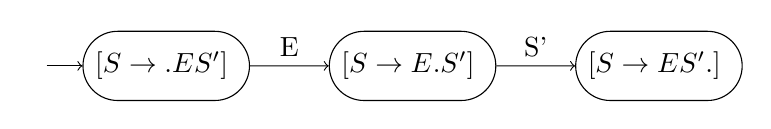
\begin{tikzpicture}[
    every text node part/.style={align=center},
    initial text =
]
    \node[state,initial]
	(S)[rounded rectangle, draw]
	{
	    {$[S \to .ES']$}
	};
    \node[state]
	(E)[rounded rectangle, draw, right=of S]
	{
	    {$[S \to E.S']$}
	};
    \node[state]
	(End)[rounded rectangle, draw, right=of E]
	{
	    {$[S \to ES'.]$}
	};

    \path[->] (S) edge  node [above] {E} (E);
    \path[->] (E) edge  node [above] {S'} (End);
\end{tikzpicture}
\]
\paragraph{Item automata for S'}
\[
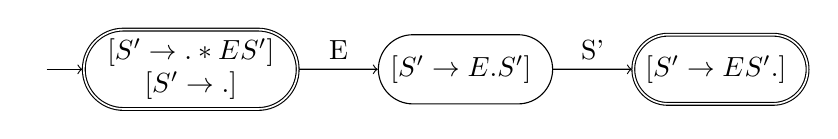
\begin{tikzpicture}[
    every text node part/.style={align=center},
    initial text =
]
    \node[state,initial,accepting]
	(S)[rounded rectangle, draw]
	{
	    {$[S'\to .*ES']$}\\
	    {$[S'\to .]$}
	};
    \node[state]
	(E)[rounded rectangle, draw,right=of S]
	{
	    {$[S'\to E.S']$}
	};
    \node[state,accepting]
	(End)[rounded rectangle, draw,right=of E]
	{
	    {$[S'\to ES'.]$}
	};
    \path[->] (S) edge  node [above] {E} (E);
    \path[->] (E) edge  node [above] {S'} (End);
\end{tikzpicture}
\]


\subsubsection{Eliminating left recursion (in EBNF Form)}

Expressing the BNF notation in EBNF reveals how the item automata for $S$ and
$S'$ can be combined in an implementation using a do-while loop:

\begin{grammar}
\underbrace{\nonterminal{expression-sequence}}_{= S}
    \produces
	\underbrace{\nonterminal{expression}}_{= E}
	\underbrace{
	\{\;
	    \nonterminal{expression}
	\}
	}_{= E'}
	\\
\end{grammar}\\[-0.5cm]
In the case the loop can terminate if the current token is
$\mathrm{Follow}(E') = \{ \lexkeyword{EOI} \}$.


\newpage\subsection{Expression}

\begin{grammar}
\underbrace{\nonterminal{expression}}_{=:E}
    \produces
	\lexkeyword{EOL} \\
    \produces
	\underbrace{\nonterminal{additive-expression}}_{=:A}
	\lexkeyword{EOL} \\
\end{grammar}

\paragraph{Item automata for E}
\[
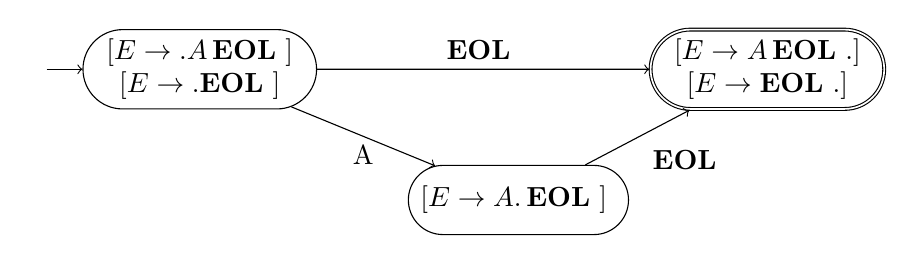
\begin{tikzpicture}[
    every text node part/.style={align=center},
    initial text =
]
    \node[state,initial]
	(S)[rounded rectangle, draw]
	{
	    {$[E \to .A\,\lexkeyword{EOL}]$}\\
	    {$[E \to .\lexkeyword{EOL}]$}
	};
    \node[state,accepting]
	(EOL)[rounded rectangle, draw, right=12em of S]
	{
	    {$[E \to A\,\lexkeyword{EOL}.]$}\\
	    {$[E \to \lexkeyword{EOL}.]$}
	};
    \node[state]
	(A)[rounded rectangle, draw, below right=2em and 6em of S]
	{
	    {$[E \to A.\,\lexkeyword{EOL}]$}
	};

    \path[->] (S) edge  node [above] {\lexkeyword{EOL}} (EOL);
    \path[->] (S) edge  node [below] {A} (A);
    \path[->] (A) edge  node [below right=0.1em and 0.2em]
	{\lexkeyword{EOL}} (EOL);
\end{tikzpicture}
\]



\newpage\subsection{Additive Expression}

\begin{grammar}
\nonterminal{additive-expression}
    \produces
	\nonterminal{multiplicative-expression} \\
    \produces
	\nonterminal{additive-expression}
	\lexkeyword{+}
	\nonterminal{multiplicative-expression} \\
    \produces
	\nonterminal{additive-expression}
	\lexkeyword{-}
	\nonterminal{multiplicative-expression} \\
\end{grammar}

\subsubsection{Eliminating left recursion}

Eliminating left recursion leads to
\begin{grammar}
\underbrace{\nonterminal{additive-expression}}_{=: A}
    \produces
	\underbrace{\nonterminal{multiplicative-expression}}_{=: M}
	\underbrace{\nonterminal{additive-expression'}}_{=:A'}\\
\nonterminal{additive-expression'}
    \produces
	\lexkeyword{+}
	\nonterminal{multiplicative-expression}
	\nonterminal{additive-expression'}
	\\
    \produces
	\lexkeyword{-}
	\nonterminal{multiplicative-expression}
	\nonterminal{additive-expression'}
	\\
    \produces
\end{grammar}\\[-0.5cm]
\noindent
The left associativity of the operators \lexkeyword{+} and \lexkeyword{-} needs
to be handled manually by the parser.

\paragraph{Item automata for A}


\[
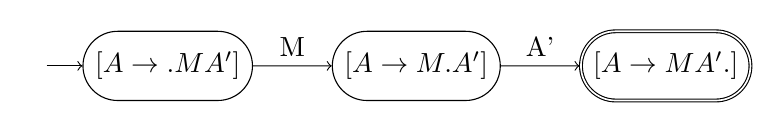
\begin{tikzpicture}[
    every text node part/.style={align=center},
    initial text =
]
    \node[state,initial]
	(S)[rounded rectangle, draw]
	{{$[A\to .MA']$}};
    \node[state]
	(M)[rounded rectangle, draw,right=of S]
	{{$[A\to M.A']$}};
    \node[state,accepting]
	(A_)[rounded rectangle, draw,right=of M]
	{{$[A\to MA'.]$}};
    \path[->] (S) edge  node [above] {M} (M);
    \path[->] (M) edge  node [above] {A'} (A_);
\end{tikzpicture}
\]

\paragraph{Item automata for A'}
\[
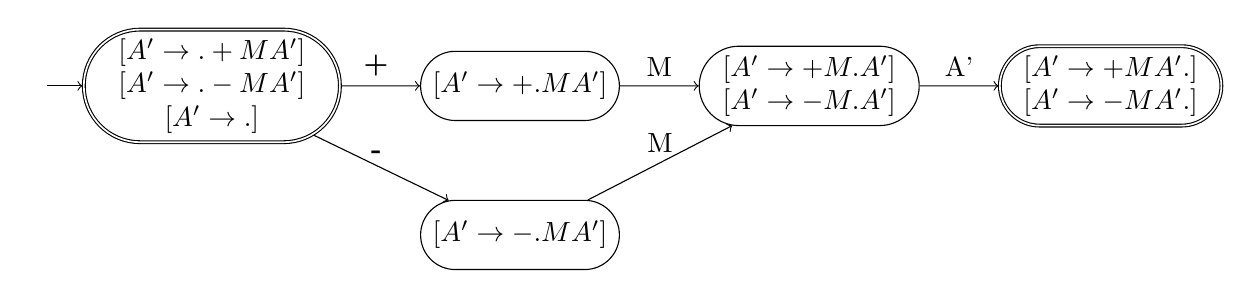
\begin{tikzpicture}[
    every text node part/.style={align=center},
    initial text =
]
    \node[state,initial,accepting]
	(S)[rounded rectangle, draw]
	{
	    {$[A'\to .+MA']$}\\
	    {$[A'\to .-MA']$}\\
	    {$[A'\to .]$}
	};
    \node[state]
	(Add)[rounded rectangle, draw,right=of S]
	{{$[A'\to +.MA']$}};
    \node[state]
	(Sub)[rounded rectangle, draw,below=of Add]
	{{$[A'\to -.MA']$}};
    \node[state]
	(M)[rounded rectangle, draw,right=of Add]
	{
	    {$[A'\to +M.A']$} \\
	    {$[A'\to -M.A']$}
	};
    \node[state,accepting]
	(E)[rounded rectangle, draw,right=of M]
	{
	    {$[A'\to +MA'.]$} \\
	    {$[A'\to -MA'.]$}
	};
    \path[->] (S) edge  node [above] {\lexkeyword{+}} (Add);
    \path[->] (S) edge  node [above] {\lexkeyword{-}} (Sub);
    \path[->] (Add) edge  node [above] {M} (M);
    \path[->] (Sub) edge  node [above] {M} (M);
    \path[->] (M) edge  node [above] {A'} (E);
\end{tikzpicture}
\]

\subsubsection{Eliminating left recursion (in EBNF Form)}

Expressing the BNF notation in EBNF reveals how the item automata for $A$ and
$A'$ can be combined in an implementation using a while loop
checking if the
current token is in $\mathrm{First}(A') = \{ \lexkeyword{+}, \lexkeyword{-}\}$:
\begin{grammar}
\underbrace{\nonterminal{additive-expression}}_{= A}
    \produces
	\underbrace{\nonterminal{multiplicative-expression}}_{= M}
	\underbrace{
	\{\;
	    \nonterminal{additive-op}
	    \nonterminal{multiplicative-expression}
	\}
	}_{=A'}
	\\
\nonterminal{additive-op}
    \produces
    \lexkeyword{+} \\
    \produces
    \lexkeyword{-} \\
\end{grammar}\\[-0.5cm]


\newpage\subsection{Multiplicative Expression}

\begin{grammar}
\nonterminal{multiplicative-expression}
    \produces
	\nonterminal{power-expression} \\
    \produces
	\nonterminal{multiplicative-expression}
	\lexkeyword{*}
	\nonterminal{power-expression} \\
    \produces
	\nonterminal{multiplicative-expression}
	\lexkeyword{/}
	\nonterminal{power-expression} \\
\end{grammar}

\subsubsection{Eliminating left recursion (in BNF Form)}

Eliminating left recursion leads to
\begin{grammar}
\underbrace{\nonterminal{multiplicative-expression}}_{=: M}
    \produces
	\underbrace{\nonterminal{power-expression}}_{=: P}
	\underbrace{\nonterminal{multiplicative-expression'}}_{=:M'}\\
\nonterminal{multiplicative-expression'}
    \produces
	\lexkeyword{*}
	\nonterminal{power-expression} \nonterminal{multiplicative-expression'}
	\\
    \produces
	\lexkeyword{/}
	\nonterminal{power-expression} \nonterminal{multiplicative-expression'}
	\\
    \produces
\end{grammar}\\[-0.5cm]
\noindent

\paragraph{Item automata for M}

\[
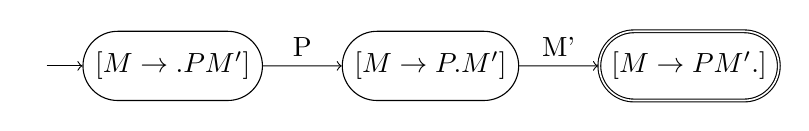
\begin{tikzpicture}[
    every text node part/.style={align=center},
    initial text =
]
    \node[state,initial]
	(S)[rounded rectangle, draw]
	{{$[M\to .PM']$}};
    \node[state]
	(P)[rounded rectangle, draw,right=of S]
	{{$[M\to P.M']$}};
    \node[state,accepting]
	(M_)[rounded rectangle, draw,right=of P]
	{{$[M\to PM'.]$}};
    \path[->] (S) edge  node [above] {P} (P);
    \path[->] (P) edge  node [above] {M'} (M_);
\end{tikzpicture}
\]

\paragraph{Item automata for M'}
\[
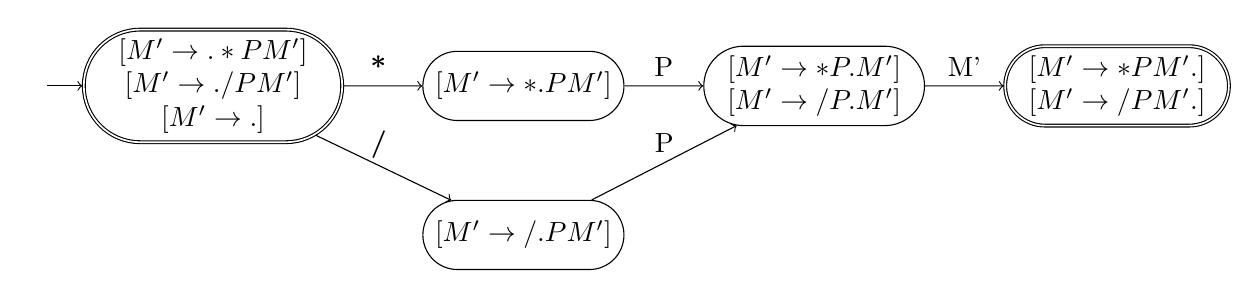
\begin{tikzpicture}[
    every text node part/.style={align=center},
    initial text =
]
    \node[state,initial,accepting]
	(S)[rounded rectangle, draw]
	{
	    {$[M'\to .*PM']$}\\
	    {$[M'\to ./PM']$}\\
	    {$[M'\to .]$}
	};
    \node[state]
	(Mul)[rounded rectangle, draw,right=of S]
	{{$[M'\to *.PM']$}};
    \node[state]
	(Div)[rounded rectangle, draw,below=of Mul]
	{{$[M'\to /.PM']$}};
    \node[state]
	(P)[rounded rectangle, draw,right=of Mul]
	{
	    {$[M'\to *P.M']$} \\
	    {$[M'\to /P.M']$}
	};
    \node[state,accepting]
	(E)[rounded rectangle, draw,right=of P]
	{
	    {$[M'\to *PM'.]$} \\
	    {$[M'\to /PM'.]$}
	};
    \path[->] (S) edge  node [above] {\lexkeyword{*}} (Mul);
    \path[->] (S) edge  node [above] {\lexkeyword{/}} (Div);
    \path[->] (Mul) edge  node [above] {P} (P);
    \path[->] (Div) edge  node [above] {P} (P);
    \path[->] (P) edge  node [above] {M'} (E);
\end{tikzpicture}
\]

\subsubsection{Eliminating left recursion (in EBNF Form)}

Expressing the BNF notation in EBNF reveals how the item automata for $M$ and
$M'$ can be combined in an implementation using a while loop
checking if the
current token is in $\mathrm{First}(M') = \{ \lexkeyword{*}, \lexkeyword{/}\}$:
\begin{grammar}
\underbrace{\nonterminal{multiplicative-expression}}_{= M}
    \produces
	\underbrace{\nonterminal{power-expression}}_{= P}
	\{\;
	\underbrace{
	    \nonterminal{multiplicative-op}
	    \nonterminal{power-expression}
	    }_{=M'}
	\}
	\\
\nonterminal{multiplicative-op}
    \produces
    \lexkeyword{*} \\
    \produces
    \lexkeyword{/} \\
\end{grammar}\\[-0.5cm]


\newpage\subsection{Power Expression}

\begin{grammar}
\underbrace{\nonterminal{power-expression}}_{=:P}
    \produces
	\underbrace{\nonterminal{unary-expression}}_{=:U} \\
    \produces
	\nonterminal{unary-expression}
	\lexkeyword{\textasciicircum}
	\nonterminal{power-expression} \\
\end{grammar}

\paragraph{Item automata for P}
\[
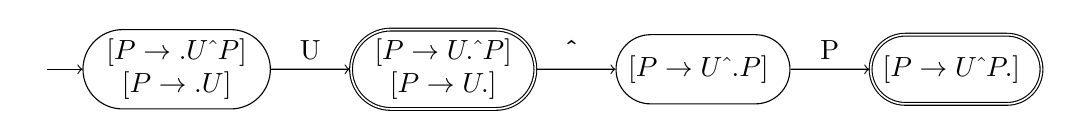
\begin{tikzpicture}[
    every text node part/.style={align=center},
    initial text =
]
    \node[state,initial]
	(S)[rounded rectangle, draw]
	{
	    {$[P\to .U\,\hat{}\, P]$} \\
	    {$[P\to .U]$}
	};
    \node[state,accepting]
	(U)[rounded rectangle, draw,right=of S]
	{
	    {$[P\to U.\,\hat{}\, P]$} \\
	    {$[P\to U.]$}
	};
    \node[state]
	(Hat)[rounded rectangle, draw,right=of U]
	{
	    {$[P\to U\,\hat{}\, .P]$}
	};
    \node[state,accepting]
	(P)[rounded rectangle, draw,right=of Hat]
	{
	    {$[P\to U\,\hat{}\, P.]$}
	};
    \path[->] (S) edge  node [above] {U} (U);
    \path[->] (U) edge  node [above] {\lexkeyword{\textasciicircum}} (Hat);
    \path[->] (Hat) edge  node [above] {P} (P);
\end{tikzpicture}
\]



\newpage\subsection{Unary Expression}

\begin{grammar}
\underbrace{\nonterminal{unary-expression}}_{=:U}
    \produces
	\underbrace{\nonterminal{primary-expression}}_{=:P} \\
    \produces
	\lexkeyword{+}
	\nonterminal{unary-expression} \\
    \produces
	\lexkeyword{-}
	\nonterminal{unary-expression} \\
\end{grammar}

\paragraph{Item automata for U}

\[
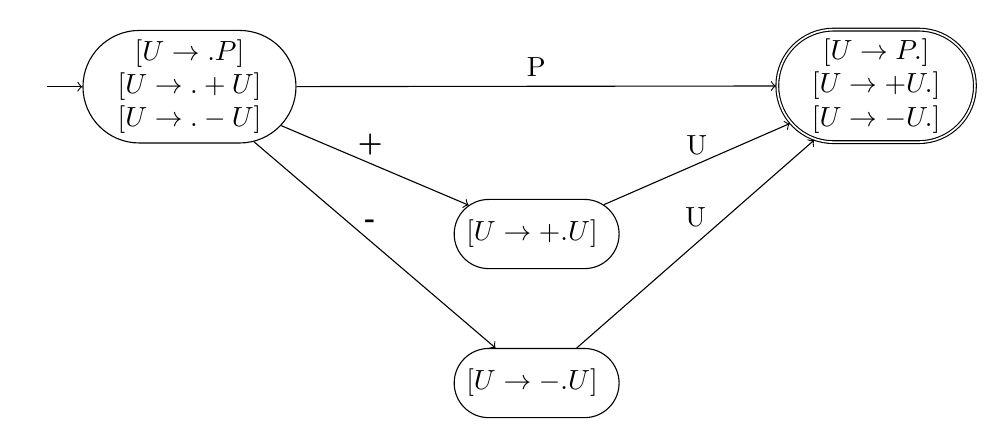
\begin{tikzpicture}[
    every text node part/.style={align=center},
    initial text =
]
    \node[state,initial]
	(S)[rounded rectangle, draw]
	{
	    {$[U\to .P]$} \\
	    {$[U\to .+U]$} \\
	    {$[U\to .-U]$}
	};
    \node[state]
	(Plus)[rounded rectangle, draw,below right=2em and 9em of S]
	{
	    {$[U\to +.U]$}
	};
    \node[state]
	(Minus)[rounded rectangle, draw,below=of Plus]
	{
	    {$[U\to -.U]$}
	};
    \node[state,accepting]
	(E)[rounded rectangle, draw,above right=2em and 9em of Plus]
	{
	    {$[U\to P.]$} \\
	    {$[U\to +U.]$} \\
	    {$[U\to -U.]$}
	};
    \path[->] (S) edge  node [above] {P} (E);
    \path[->] (S) edge  node [above] {\lexkeyword{+}} (Plus);
    \path[->] (S) edge  node [above=0.1cm] {\lexkeyword{-}} (Minus);
    \path[->] (Plus) edge  node [above] {U} (E);
    \path[->] (Minus) edge  node [above=0.1cm] {U} (E);
\end{tikzpicture}
\]


\newpage\subsection{Primary Expression}

\begin{grammar}
\underbrace{\nonterminal{primary-expression}}_{=:P}
    \produces
	\underbrace{\nonterminal{float-literal}}_{=:F} \\
    \produces
	\lexkeyword{(}
	\underbrace{\nonterminal{additive-expression}}_{=:A}
	\lexkeyword{)}\\
\end{grammar}

\paragraph{Item automata for P}
\[
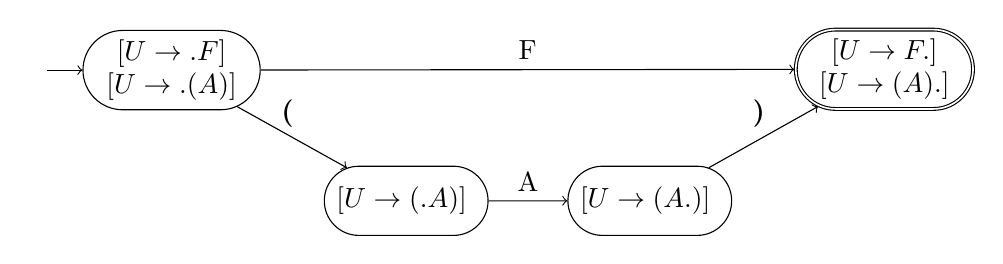
\begin{tikzpicture}[
    every text node part/.style={align=center},
    initial text =
]
    \node[state,initial]
	(S)[rounded rectangle, draw]
	{
	    {$[U\to .F]$} \\
	    {$[U\to .(A)]$}
	};
    \node[state]
	(LP)[rounded rectangle, draw,below right=2em and 5em of S]
	{
	    {$[U\to (.A)]$}
	};
    \node[state]
	(A)[rounded rectangle, draw,right=of LP]
	{
	    {$[U\to (A.)]$}
	};
    \node[state,accepting]
	(E)[rounded rectangle, draw,above right=2em and 5em of A]
	{
	    {$[U\to F.]$} \\
	    {$[U\to (A).]$}
	};
    \path[->] (S) edge  node [above] {F} (E);
    \path[->] (S) edge  node [above] {\lexkeyword{(}} (LP);
    \path[->] (LP) edge  node [above] {A} (A);
    \path[->] (A) edge  node [above] {\lexkeyword{)}} (E);
\end{tikzpicture}
\]





\end{document}
